\documentclass[handout]{beamer}
\title{Parallelle Metaheuristieken}
\author{Willem Van Onsem\\Promotor: prof. Bart Demoen}
\date{27 maart 2013}
\usepackage{tikz,amsfonts,amsmath}
\usetikzlibrary{shapes,calc}
\usepackage[dutch]{babel}
\usetheme{Antibes}
\newcommand{\sol}{\mathcal{S}}
\newcommand{\constr}{\mathcal{C}}
\newcommand{\RR}{\mathbb{R}}
\begin{document}
\begin{frame}
\maketitle
\end{frame}
\begin{frame}
\tableofcontents
\end{frame}
\section{Inleiding}
\begin{frame}{Inleiding}
\begin{itemize}[<+->]
 \item Belangrijk onderwerp in AI: optimalisatieproblemen
 \item Meestal NP-hard dus intractable
 \item Heuristieken bieden ``oplossing'', maar:
 \begin{itemize}[<+->]
  \item afhankelijk van instantie
  \item meestal niet aanpasbaar naar gegeven tijd,...
 \end{itemize}
 \item Meer aanpasbaar: Metaheuristieken
\end{itemize}
\end{frame}
\subsection{Metaheuristieken}
\begin{frame}{Inleiding: Metaheuristieken}
\begin{itemize}[<+->]
 \item Oplossingsruimte $\sol$
 \item Begin met een ``toevallige'' oplossing $s\in\sol$
 \item Voer sequentie van metaheuristieken uit
 \begin{equation}
  h_i:\sol^{k_i}\rightarrow\sol
 \end{equation}
 \item Herhalen tot tijd op is
 \item Beste oplossing tot dusver onthouden en teruggeven
 \item Populaire implementaties:
 \begin{itemize}[<+->]
   \item Genetische algoritmen
   \item Simulated Annealing
   \item ...
 \end{itemize}
 \item Research: ``Operational Research''
\end{itemize}
\end{frame}
\subsection{HyFlex}
\begin{frame}{Inleiding: \emph{HyFlex}}
\begin{itemize}[<+->]
 \item Enkele formele modellen
 \item Tot dusver vooral probleemafhankelijk denken
 \item Belangrijk: $h_i$-functies
 \item Naar algemene oplossingsmethodes: Hyperheuristieken
 \begin{itemize}
   \item Ontwikkel grote collectie van $h_i$-functies
   \item Laat een algemeen probleemonafhankelijk systeem kiezen welke $h_i$ toe te passen
 \end{itemize}
 \item Implementatie voor research: \emph{HyFlex}
 \item Competitie in 2011: \emph{CHeSC2011}
\end{itemize}
\end{frame}
\begin{frame}{Inleiding: \emph{HyFlex}}
\begin{figure}
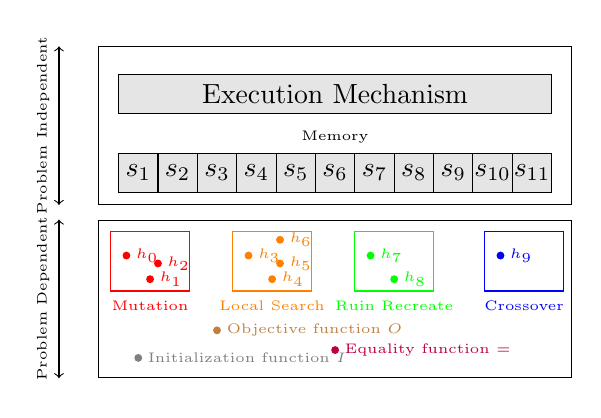
\begin{tikzpicture}
\node[draw,rectangle,minimum width=6 cm, minimum height=2cm] (PI) at (0,1.1) {};
\node[draw,rectangle,minimum width=6 cm, minimum height=2cm] (PD) at (0,-1.1) {};
\coordinate (PDL) at ($(PD.north west)+(-0.5,0)$);
\coordinate (PIL) at ($(PI.north west)+(-0.5,0)$);
\draw[<->] (PDL |- PD.south west) to node[above,midway,sloped]{\tiny{Problem Dependent}} (PDL);
\draw[<->] (PIL |- PI.south west) to node[above,midway,sloped]{\tiny{Problem Independent}} (PIL);
\begin{scope}[red]
  \node[draw,rectangle,minimum width=1cm, minimum height=0.75cm] (LL1) at (-2.35,-0.625) {};
  \fill (-2.65,-0.55) circle (0.05cm) node[anchor=west] {\tiny{$h_0$}};
  \fill (-2.35,-0.85) circle (0.05cm) node[anchor=west] {\tiny{$h_1$}};
  \fill (-2.25,-0.65) circle (0.05cm) node[anchor=west] {\tiny{$h_2$}};
  \draw (LL1.south) node[anchor=north] {\tiny{Mutation}};
\end{scope}
\begin{scope}[xshift=1.55 cm,orange]
  \node[draw,rectangle,minimum width=1cm, minimum height=0.75cm] (LL2) at (-2.35,-0.625) {};
  \fill (-2.65,-0.55) circle (0.05cm) node[anchor=west] {\tiny{$h_3$}};
  \fill (-2.35,-0.85) circle (0.05cm) node[anchor=west] {\tiny{$h_4$}};
  \fill (-2.25,-0.65) circle (0.05cm) node[anchor=west] {\tiny{$h_5$}};
  \fill (-2.25,-0.35) circle (0.05cm) node[anchor=west] {\tiny{$h_6$}};
  \draw (LL2.south) node[anchor=north] {\tiny{Local Search}};
\end{scope}
\begin{scope}[xshift=3.1 cm,green]
  \node[draw,rectangle,minimum width=1cm, minimum height=0.75cm] (LL3) at (-2.35,-0.625) {};
  \fill (-2.65,-0.55) circle (0.05cm) node[anchor=west] {\tiny{$h_7$}};
  \fill (-2.35,-0.85) circle (0.05cm) node[anchor=west] {\tiny{$h_8$}};
  \draw (LL3.south) node[anchor=north] {\tiny{Ruin Recreate}};
\end{scope}
\begin{scope}[xshift=4.75 cm,blue]
  \node[draw,rectangle,minimum width=1cm, minimum height=0.75cm] (LL4) at (-2.35,-0.625) {};
  \fill (-2.65,-0.55) circle (0.05cm) node[anchor=west] {\tiny{$h_9$}};
  \draw (LL4.south) node[anchor=north] {\tiny{Crossover}};
\end{scope}
\fill[purple] (0,-1.75) circle (0.05cm) node[anchor=west] {\tiny{Equality function $=$}};
\fill[brown] (-1.5,-1.5) circle (0.05cm) node[anchor=west] {\tiny{Objective function $O$}};
\fill[gray] (-2.5,-1.85) circle (0.05cm) node[anchor=west] {\tiny{Initialization function $I$}};
\node[draw,rectangle,fill=gray!20,minimum width=5.5 cm, minimum height=0.5cm] (MEM) at (0,0.5) {};
\foreach\x in {-2.25,-1.75,...,2.25} {
  \draw (\x,0.25) -- ++(0,0.5);
}
\foreach\x in {1,2,...,11} {
  \draw (-2.75+0.5*\x-0.25,0.5) node {$s_{\x}$};
}
\draw (MEM.north) node[anchor=south] {\tiny{Memory}};
\node[draw,rectangle,fill=gray!20,minimum width=5.5 cm, minimum height=0.5cm] (EXC) at (0,1.5) {Execution Mechanism};
\end{tikzpicture}
\caption{Structuur van \emph{HyFlex}}
\end{figure}
\end{frame}
\section{ParHyFlex}
\begin{frame}{\emph{ParHyFlex}}
Doel: Ontwikkelen van Parallelle variant: \emph{ParHyFlex}
\begin{itemize}[<+->]
 \item Elke machine houdt een oplossingsruimte bij
 \item Gebruikers ontwikkelen (sequenti\"ele) hyperheuristieken
 \item \emph{ParHyFlex}: zorgt voor uitvoering met goede speedup
 \item Belangrijk: Intensification-Diversification cycle
 \begin{itemize}[<+->]
  \item Intensification: ``goede concepten'' delen
  \item Diversification: niet in elkaars ``vaarwater'' zitten
 \end{itemize}
 \item Extra low-level features:
 \begin{itemize}[<+->]
  \item Afstandsfuncties $\delta_i:\sol^2\rightarrow\RR$
  \item Afdwingbare constraints: $c_i:\sol\rightarrow\sol$
  \item Hypothese generatoren: $g_i:\sol^k\rightarrow\constr:\sol^k\rightarrow\left(\sol\rightarrow\sol\right)$
  \item Meerdere (virtuele) objectieven: $O_i:\sol\rightarrow\RR$
 \end{itemize}
\end{itemize}
\end{frame}
\subsection{Structuur}
\begin{frame}{\emph{ParHyFlex}: Structuur}
\begin{figure}
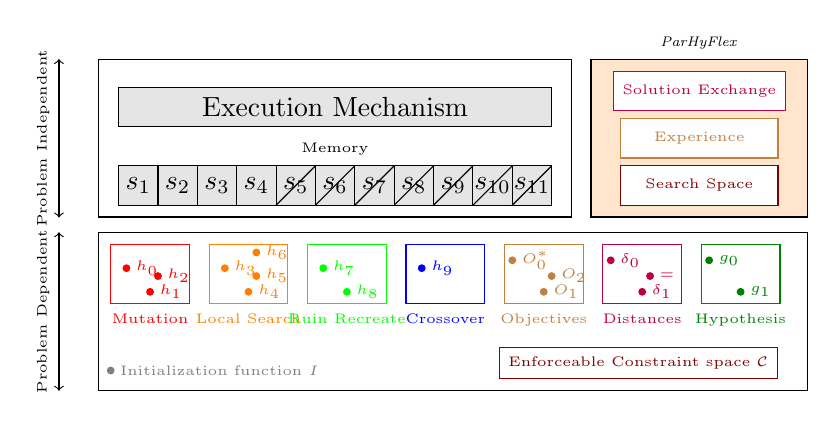
\begin{tikzpicture}
\node[draw,rectangle,minimum width=6 cm, minimum height=2cm] (PI) at (-1.5,1.1) {};
\node[draw,rectangle,fill=orange!20,minimum width=2.75 cm, minimum height=2cm] (PH) at (3.125,1.1) {};
\node[draw,rectangle,minimum width=9 cm, minimum height=2cm] (PD) at (0,-1.1) {};
\coordinate (PDL) at ($(PD.north west)+(-0.5,0)$);
\coordinate (PIL) at ($(PI.north west)+(-0.5,0)$);
\draw[<->] (PDL |- PD.south west) to node[above,midway,sloped]{\tiny{Problem Dependent}} (PDL);
\draw[<->] (PIL |- PI.south west) to node[above,midway,sloped]{\tiny{Problem Independent}} (PIL);
\begin{scope}[red,xshift=-0.5 cm]
  \node[draw,rectangle,minimum width=1cm, minimum height=0.75cm] (LL1) at (-3.35,-0.625) {};
  \fill (-3.65,-0.55) circle (0.05cm) node[anchor=west] {\tiny{$h_0$}};
  \fill (-3.35,-0.85) circle (0.05cm) node[anchor=west] {\tiny{$h_1$}};
  \fill (-3.25,-0.65) circle (0.05cm) node[anchor=west] {\tiny{$h_2$}};
  \draw (LL1.south) node[anchor=north] {\tiny{Mutation}};
\end{scope}
\begin{scope}[xshift=0.75 cm,orange]
  \node[draw,rectangle,minimum width=1cm, minimum height=0.75cm] (LL2) at (-3.35,-0.625) {};
  \fill (-3.65,-0.55) circle (0.05cm) node[anchor=west] {\tiny{$h_3$}};
  \fill (-3.35,-0.85) circle (0.05cm) node[anchor=west] {\tiny{$h_4$}};
  \fill (-3.25,-0.65) circle (0.05cm) node[anchor=west] {\tiny{$h_5$}};
  \fill (-3.25,-0.35) circle (0.05cm) node[anchor=west] {\tiny{$h_6$}};
  \draw (LL2.south) node[anchor=north] {\tiny{Local Search}};
\end{scope}
\begin{scope}[xshift=2 cm,green]
  \node[draw,rectangle,minimum width=1cm, minimum height=0.75cm] (LL3) at (-3.35,-0.625) {};
  \fill (-3.65,-0.55) circle (0.05cm) node[anchor=west] {\tiny{$h_7$}};
  \fill (-3.35,-0.85) circle (0.05cm) node[anchor=west] {\tiny{$h_8$}};
  \draw (LL3.south) node[anchor=north] {\tiny{Ruin Recreate}};
\end{scope}
\begin{scope}[xshift=3.25 cm,blue]
  \node[draw,rectangle,minimum width=1cm, minimum height=0.75cm] (LL4) at (-3.35,-0.625) {};
  \fill (-3.65,-0.55) circle (0.05cm) node[anchor=west] {\tiny{$h_9$}};
  \draw (LL4.south) node[anchor=north] {\tiny{Crossover}};
\end{scope}
\begin{scope}[xshift=4.5 cm,brown]
  \node[draw,rectangle,minimum width=1cm, minimum height=0.75cm] (OBJ) at (-3.35,-0.625) {};
  \fill (-3.75,-0.45) circle (0.05cm) node[anchor=west] {\tiny{$O_0^*$}};
  \fill (-3.35,-0.85) circle (0.05cm) node[anchor=west] {\tiny{$O_1$}};
  \fill (-3.25,-0.65) circle (0.05cm) node[anchor=west] {\tiny{$O_2$}};
  \draw (OBJ.south) node[anchor=north] {\tiny{Objectives}};
\end{scope}
\begin{scope}[xshift=5.75 cm,purple]
  \node[draw,rectangle,minimum width=1cm, minimum height=0.75cm] (DIS) at (-3.35,-0.625) {};
  \fill (-3.75,-0.45) circle (0.05cm) node[anchor=west] {\tiny{$\delta_0$}};
  \fill (-3.35,-0.85) circle (0.05cm) node[anchor=west] {\tiny{$\delta_1$}};
  \fill (-3.25,-0.65) circle (0.05cm) node[anchor=west] {\tiny{$=$}};
  \draw (DIS.south) node[anchor=north] {\tiny{Distances}};
\end{scope}
\begin{scope}[xshift=7 cm,green!50!black]
  \node[draw,rectangle,minimum width=1cm, minimum height=0.75cm] (DIS) at (-3.35,-0.625) {};
  \fill (-3.75,-0.45) circle (0.05cm) node[anchor=west] {\tiny{$g_0$}};
  \fill (-3.35,-0.85) circle (0.05cm) node[anchor=west] {\tiny{$g_1$}};
  \draw (DIS.south) node[anchor=north] {\tiny{Hypothesis}};
\end{scope}
\fill[gray] (-4.35,-1.85) circle (0.05cm) node[anchor=west] {\tiny{Initialization function $I$}};
\node[red!50!black,draw,rectangle] at (2.35,-1.75) {\tiny{Enforceable Constraint space $\constr$}};
\begin{scope}[xshift=-1.5 cm]
  \node[draw,rectangle,fill=gray!20,minimum width=5.5 cm, minimum height=0.5cm] (MEM) at (0,0.5) {};
  \foreach\x in {-2.25,-1.75,...,2.25} {
    \draw (\x,0.25) -- ++(0,0.5);
  }
  \foreach\x in {-0.75,-0.25,...,2.25} {
    \draw (\x,0.25) -- ++(0.5,0.5);
  }
  \foreach\x in {1,2,...,11} {
    \draw (-2.75+0.5*\x-0.25,0.5) node {$s_{\x}$};
  }
  \draw (MEM.north) node[anchor=south] {\tiny{Memory}};
  \node[draw,rectangle,fill=gray!20,minimum width=5.5 cm, minimum height=0.5cm] (EXC) at (0,1.5) {Execution Mechanism};
\end{scope}
\draw (PH.north) node[anchor=south] {\tiny{\emph{ParHyFlex}}};
\node[draw,brown,fill=white,rectangle,minimum width=2 cm, minimum height=0.5 cm] at (3.125,1.1) {\tiny{Experience}};
\node[draw,purple,fill=white,rectangle,minimum width=2 cm, minimum height=0.5 cm] at (3.125,1.7) {\tiny{Solution Exchange}};
\node[draw,red!50!black,fill=white,rectangle,minimum width=2 cm, minimum height=0.5 cm] at (3.125,0.5) {\tiny{Search Space}};
\end{tikzpicture}
\caption{Structuur van \emph{ParHyFlex}}
\end{figure}
\end{frame}
\subsection{Werking}
\begin{frame}{\emph{ParHyFlex}: Werking}
\begin{figure}
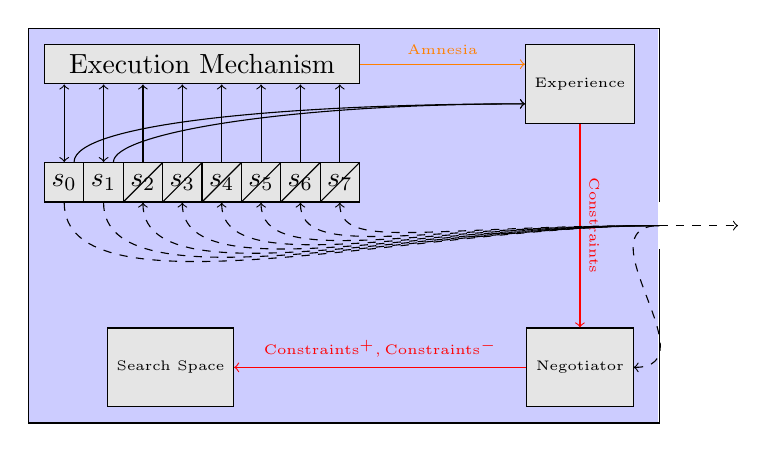
\begin{tikzpicture}
\node[draw=white,rectangle,minimum width=8 cm, minimum height=5 cm,fill=blue!20] (Machine) at (0,0) {};
\draw[black] ($(Machine.east)+(0,0.3)$) -- (Machine.north east) -| (Machine.south west) -| ($(Machine.east)+(0,-0.3)$);
\coordinate (OC) at (Machine.east);
\draw[dashed,->] (OC) -- ++(1,0);
\node[draw,rectangle,fill=gray!20,minimum width=4 cm, minimum height=0.5cm] (EXC) at (-1.8,2.05) {Execution Mechanism};
\node[draw,rectangle,fill=gray!20,minimum width=1 cm, minimum height=1cm] (EXP) at (3,1.8) {\tiny{Experience}};
\draw[orange,->] (EXC.east) to node[above]{\tiny Amnesia} (EXP.west |- EXC.east);
\node[draw,rectangle,fill=gray!20,minimum width=1 cm, minimum height=1cm] (NGT) at (3,-1.8) {\tiny{Negotiator}};
\draw[red,->] (EXP) to node[above,sloped]{\tiny Constraints} (NGT);
\draw[dashed,<-] (NGT.east) .. controls ($(NGT.east)+(1,0)$) and ($(OC)+(-1,0)$) .. (OC);
\node[draw,rectangle,fill=gray!20,minimum width=1 cm, minimum height=1cm] (SSP) at (-2.2,-1.8) {\tiny{Search Space}};
\draw[red,->] (NGT) to node[above,sloped]{\tiny $\mbox{Constraints}^+,\mbox{Constraints}^-$} (SSP);

\begin{scope}[xshift=-1.8 cm,yshift=0.55cm]
\node[draw,rectangle,fill=gray!20,minimum width=4 cm, minimum height=0.5cm] (MEM) at (0,0) {};
\foreach\x in {-1.5,-1,...,1.5} {
  \draw (\x,-0.25) -- ++(0,0.5);
}
\foreach\x in {-1,-0.5,...,1.5} {
  \draw (\x,-0.25) -- ++(0.5,0.5);
}
\foreach\x in {0,1} {
  \draw (0.5*\x-1.75,0) node {$s_{\x}$};
  \draw[<->] (MEM.north -| 0.5*\x-1.75,0) -- (EXC.south -| 0.5*\x-1.75,0);
  \draw[dashed] (MEM.south -| 0.5*\x-1.75,0) .. controls (0.5*\x-1.75,0.125*\x-1.75) and ($(OC)+(-3,0)$) .. (OC);
  \draw[->] (MEM.north -| 0.5*\x-1.625,0) .. controls (0.5*\x-1.625,-0.125*\x+0.75) and ($0.5*(EXP.west)+0.5*(EXP.south west)+(-3,0)$) .. ($0.5*(EXP.west)+0.5*(EXP.south west)$);
}
\foreach\x in {2,3,...,7} {
  \draw (0.5*\x-1.75,0) node {$s_{\x}$};
  \draw[->] (MEM.north -| 0.5*\x-1.75,0) -- (EXC.south -| 0.5*\x-1.75,0);
  \draw[<-,dashed] (MEM.south -| 0.5*\x-1.75,0) .. controls (0.5*\x-1.75,0.125*\x-1.75) and ($(OC)+(-3,0)$) .. (OC);
}
\end{scope}
\end{tikzpicture}
\caption{Werking van \emph{ParHyFlex}}
\end{figure}
\end{frame}
\begin{frame}{\emph{ParHyFlex}: Werking}
\begin{figure}
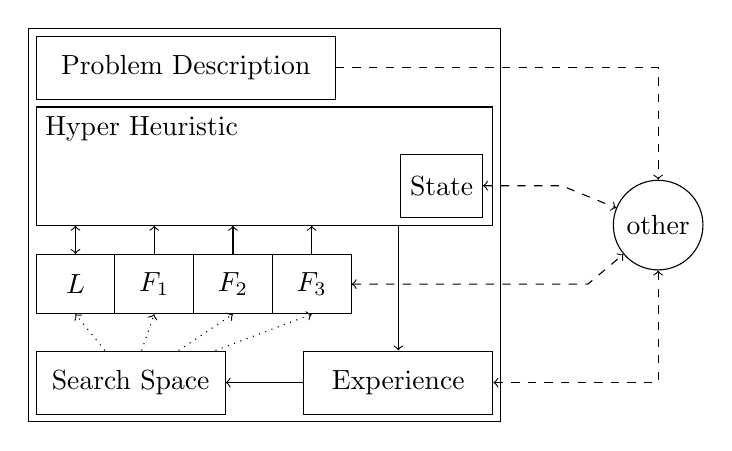
\begin{tikzpicture}
\node[draw,rectangle,minimum width=6cm,minimum height=5cm] (S) at (0,0) {};
\node[draw,rectangle,minimum width=3.8cm,minimum height=0.8cm] (P) at (-1,2) {Problem Description};
\node[draw,rectangle,minimum width=5.8cm,minimum height=1.5cm] (HH) at (0,0.75) {};
\node[draw,rectangle,minimum width=4cm,minimum height=0.75cm] (MEM) at (-0.9,-0.75) {};
\node[draw,rectangle,minimum width=2.4cm,minimum height=0.8cm] (EX) at (1.7,-2) {Experience};
\node[draw,rectangle,minimum width=2.4cm,minimum height=0.8cm] (SS) at (-1.7,-2) {Search Space};
\node[draw,rectangle,minimum width=0.8cm,minimum height=0.8cm] (HHS) at (2.25,0.5) {State};
\node[draw,circle] (O) at (5,0) {other};

\foreach \b in {1,2,3} {
  \draw (\b-2.9,0 |- MEM.north) -- (\b-2.9,0 |- MEM.south);
}

\foreach \b/\t in {0/$L$,1/$F_1$,2/$F_2$,3/$F_3$} {
  \node[minimum width=1cm,minimum height=0.75cm] (M\b) at (\b-2.4,0 |- MEM.east) {\t};
  \draw[dotted,->] (SS) -- (M\b.south);
}

\node[anchor=north west] at (HH.north west) {Hyper Heuristic};

\draw[dashed,->] (P) -| (O);
\draw[dashed,<->] (EX) -| (O);
\draw[dashed,<->] (MEM.east) -- ++(3,0) -- (O);
\draw[dashed,<->] (HHS.east) -- ++(1,0) -- (O);
\draw[->] (HH.south -| EX) -- (EX);
\draw[->] (EX) -- (SS);

\draw[<->] (M0.north) -- (M0 |- HH.south);
\draw[->] (M1.north) -- (M1 |- HH.south);
\draw[->] (M2.north) -- (M2 |- HH.south);
\draw[->] (M3.north) -- (M3 |- HH.south);
\end{tikzpicture}
\caption{Werking van \emph{ParHyFlex}}
\end{figure}
\end{frame}
\subsection{Componenten}
\begin{frame}{\emph{ParHyFlex}: Componenten}
\emph{Problem Description} component:
\begin{itemize}[<+->]
 \item Metaprobleem overal gekend
 \item Specifiek probleem aanmaken op \emph{root}
 \item Broadcast naar andere machines
\end{itemize}
\emph{Geheugen} component:
\begin{itemize}[<+->]
 \item Slaat tussen-oplossingen op
 \item Lokaal lees-schrijf geheugen
 \item Vreemd lees geheugen
 \item Bewaakt door \emph{Search Space}
 \item Met uitwisselingsstrategie (reduceren van bandbreedte)
\end{itemize}
\end{frame}
\begin{frame}{ParHyFlex: Structuur}
\emph{Experience} component:
\begin{itemize}[<+->]
 \item Vat zoekervaring samen
 \item Wisselt ervaring uit met andere machines
 \item Onderhandelt over nieuwe zoekruimte
 \item Past de actieve zoekruimte aan
 \item Eenheid: \emph{Enforceable Constraints}
 \item Amnesie implementeren
\end{itemize}
\emph{Search Space} component:
\begin{itemize}[<+->]
 \item Bewaakt de zoekruimte
 \item Past gegenereerde/ontvangen oplossingen aan
 \item Met behulp van \emph{Enforceable Constraints}
 \item Standaard: Positieve set, Negatieve Set
 \item Constraints worden \emph{fuzzy} afgedwongen
\end{itemize}
\end{frame}
\section{Probleem: 3SAT}
\begin{frame}{Probleem: MAX3SAT}
\begin{itemize}[<+->]
 \item Prestaties framework testen op MAX3SAT
 \item Booleaanse optimalisatie
 \item Motivering:
 \begin{itemize}[<+->]
  \item Eenvoudig probleem
  \item Veel bestaand onderzoek
  \item Veel aspecten \emph{inherent}
  \item NP-hard (andere problemen omzetten)
 \end{itemize}
\end{itemize}
\end{frame}
\subsection{Componenten}
\begin{frame}{Probleem: MAX3SAT: Componenten}
\emph{Experience} component:
\begin{itemize}[<+->]
 \item Clause learner
 \item Genereren van clauses die waar zijn voor een oplossing
 \item Evaluatie op andere oplossingen
 \item Variabelen in clause toevallig volgens verdeling
 \begin{equation}
  p(x_i)=(n_i^++n_i^-)\cdot -(p_i^+\log p_i^++p_i^-\log p_i^-)
 \end{equation}
 \item Amnesie: verwijderen van clauses
 \item Merk op: Clause is een \emph{Enforceable Constraint}
 \item Onderhandeling: andere machines plaatsen clauses in negatieve search space, en ervaring set
\end{itemize}
\end{frame}
\subsection{Probleemafhankelijke Componenten}
\section{Communicatie}
\begin{frame}{Communicatie}
\begin{itemize}[<+->]
 \item Parallelle bibliotheken gericht op computationele problemen
 \item Voorbeeld: Sorteren, Matrix-vermenigvuldiging
 \item Communicatie (aangepaste \emph{TCP})
 \begin{itemize}[<+->]
  \item Betrouwbaar
  \item Synchroon (\emph{MPI}: optioneel)
  \item Sequenti\"eel (niet bij \emph{Tuple Space})
  \item Atomair
 \end{itemize}
 \item Niet ideaal voor het uitwisselen van oplossingen
 \item Hoge kostprijs (zie verder)
 \item Idee: sommige communicatie over \emph{UDP}
\end{itemize}
\end{frame}
\subsection{Betrouwbaar}
\begin{frame}{Communicatie: Betrouwbaar}
Betrouwbare communicatie?
\begin{itemize}[<+->]
 \item Parallelle setting: meestal goede verbinding
 \item Geen bewijs dat uitwisseling altijd iets oplevert
 \item Kost van betrouwbaarheid:
 \begin{itemize}[<+->]
  \item \emph{ACK}-bericht
  \item Heruitsturen (na timeout!)
  \item Netwerk blijft ``outdated berichten sturen''
 \end{itemize}
 \item Voordeel \emph{UDP}:
 \begin{itemize}
  \item Minder bandbreedte
  \item Netwerk als buffer tegen verzadiging
 \end{itemize}
\end{itemize}
\end{frame}
\subsection{Synchroon}
\begin{frame}{Communicatie: Sequentieel}
Synchroon communicatie?
\begin{itemize}[<+->]
 \item Hyperheuristiek en onderliggende heuristieken divers
 \item Kans om op hetzelfde moment barri\`ere tegen te komen nihiel
 \item Wachten zorgt voor ineffici\"ent CPU-gebruik
 \item Betere strategie: uitsturen en meteen verder werken
 \item ref. \emph{IDP} bevat assynchrone directieven
\end{itemize}
\end{frame}
\subsection{Sequenti\"eel}
\begin{frame}{Communicatie: Sequentieel}
Sequentie\"ele communicatie?
\begin{itemize}[<+->]
 \item We willen geheugen telkens up-to-date houden
 \item Oplossing uitwisselen indien reeds herzien?
 \item Levert extra bandbreedte op
 \item ref. \emph{Tuple Space} paradigma's
 \item Nadeel: actuelere oplossing niet altijd ``betere''
\end{itemize}
\end{frame}
\subsection{Atomair}
\begin{frame}{Communicatie: Atomair}
Atomaire communicatie?
\begin{itemize}[<+->]
 \item Diverse communicatie (oplossingen, ervaring, toestand)
 \item Verschillende prioriteiten
 \item Kost van bericht: bericht zelf, aantal bytes minder relevant
 \item Idee: opsparen van berichten en meesturen met anderen
 \item ref. \emph{Piggybacking} van \emph{ACK} in \emph{TCP}
\end{itemize}
\end{frame}
\end{document}
